% Author: Izaak Neutelings (March 2020)
\documentclass[border=3pt,tikz]{standalone}
\usepackage{amsmath} % for \dfrac
\usepackage{bm} % \bm
\usepackage{physics}
\usepackage{tikz,pgfplots}
\usepackage[outline]{contour} % glow around text
\usetikzlibrary{angles,quotes} % for pic (angle labels)
\usetikzlibrary{calc}
\usetikzlibrary{decorations.markings}
\usetikzlibrary{patterns,snakes}
\tikzset{>=latex} % for LaTeX arrow head
\contourlength{1.6pt}
\usepackage{xcolor}
\colorlet{Bcol}{violet!90}
\colorlet{BFcol}{red!60!black}
\colorlet{veccol}{green!45!black}
\colorlet{Icol}{blue!70!black}
\tikzstyle{BField}=[->,thick,Bcol!70!black]
\tikzstyle{BFieldLineArrowless}=[->,thick,Bcol]
\tikzstyle{current}=[->,Icol] %thick,
\tikzstyle{force}=[->,thick,BFcol]
\tikzstyle{vector}=[->,thick,veccol!70!black]
\tikzstyle{velocity}=[->,thick,veccol]
\tikzstyle{charge+}=[very thin,draw=black,top color=red!50,bottom color=red!90!black,shading angle=20,circle,inner sep=0.5]
\tikzstyle{charge-}=[very thin,draw=black,top color=blue!50,bottom color=blue!80,shading angle=20,circle,inner sep=0.5]
\tikzstyle{metal}=[top color=black!15,bottom color=black!25,middle color=black!5,shading angle=10]
\tikzset{
  BFieldLine/.style={thick,Bcol,decoration={markings,mark=at position #1 with {\arrow{latex}}},
                                 postaction={decorate}},
  BFieldLine/.default=0.5,
  pics/Bin/.style={
    code={
      \def\R{0.12}
      \draw[pic actions,line width=0.6,#1] % ,thick
        (0,0) circle (\R) (-135:.75*\R) -- (45:.75*\R) (-45:.75*\R) -- (135:.75*\R);
  }},
  pics/Bout/.style={
    code={
      \def\R{0.12}
      \draw[pic actions,line width=0.6,#1,fill=white] (0,0) circle (\R);
      \fill[pic actions,#1] (0,0) circle (0.3*\R);
  }},
  pics/Bin/.default=Bcol,
  pics/Bout/.default=Bcol,
}



\begin{document}


% CURRENT IN B FIELD
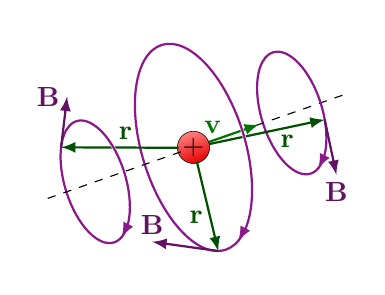
\begin{tikzpicture}[z={(0.8,0.28)},x={(0.62,-0.45)}]
  \def\R{1.2}
  \def\ang{-40}
  \def\scale{1.3}
  \def\Rscaled{\R/\scale^2}
  \coordinate (O) at (0,0,0);
  \coordinate (L) at (0,0,-\scale*\R);
  \coordinate (R) at (0,0, \scale*\R);
  \coordinate (LB) at ({\Rscaled*cos(170)},{\Rscaled*sin(170)},-\scale*\R);
  \coordinate (RB) at ({\Rscaled*cos(18)},{\Rscaled*sin(18)}, \scale*\R);
  %\draw (0,0,0) -- (2,0,0);
  %\draw (0,0,0) -- (0,0,2);
  
  % B FIELD
  \draw[BFieldLineArrowless,-] (O)++(\ang+1:\R) arc (\ang+1:\ang-181:\R);
  \draw[BFieldLineArrowless,-] (L)++(\ang+1:\R/\scale^2) arc (\ang+1:\ang-181:\R/\scale^2);
  \draw[BFieldLineArrowless,-] (R)++(\ang+1:\R/\scale^2) arc (\ang+1:\ang-181:\R/\scale^2);
  %\draw[BField,-] (0,0,-2*\scale*\R)++(\ang+1:\R/\scale^2/4) arc (\ang+1:\ang-181:\R/\scale^2/4);
  %\draw[BField,-] (0,0, 2*\scale*\R)++(\ang+1:\R/\scale^2/4) arc (\ang+1:\ang-181:\R/\scale^2/4);
  
  % CHARGE
  \draw[dashed] (O) -- (0,0,2.0*\R);
  \draw[vector] (O) -- (RB) node[midway,right=7,below right=-3,scale=1] {$\vb{r}$};
  \draw[velocity] (O) -- (0,0,1.04) node[midway,left=1,above left=-3] {$\vb{v}$};
  \node[charge+] %draw=black,circle,fill,inner sep=1,scale=0.6
    (O) at (O) {$+$};
  \draw[dashed] (O)++(0,0,-0.2) -- (0,0,-2.0*\R);
  
  % B FIELD
  \draw[vector] (O)++(-155:0.28*\R) -- (LB) node[midway,right=2,above=-1,scale=1] {$\vb{r}$};
  \draw[white,very thick] (O)++(\ang+179:\R) arc (\ang+179:\ang+1:\R);
  \draw[white,very thick] (L)++(\ang+179:\R/\scale^2) arc (\ang+179:\ang+1:\R/\scale^2);
  \draw[BFieldLine=1] (O)++(\ang+180:\R) arc (\ang+180:\ang:\R) --++ (-122:0.001*\R);
  \draw[BFieldLine=1] (L)++(\ang+180:\R/\scale^2) arc (\ang+180:\ang:\R/\scale^2) --++ (-120:0.001*\R);
  \draw[BFieldLine=1] (R)++(\ang+180:\R/\scale^2) arc (\ang+180:\ang:\R/\scale^2) --++ (-120:0.001*\R);
  %\draw[BFieldLine=1] (0,0,-2*\scale*\R)++(\ang+180:\R/\scale^2/4) arc (\ang+180:\ang:\R/\scale^2/4) --++ (58:0.01*\R);
  %\draw[BFieldLine=1] (0,0, 2*\scale*\R)++(\ang+180:\R/\scale^2/4) arc (\ang+180:\ang:\R/\scale^2/4) --++ (58:0.01*\R);
  
  \draw[vector] (O)++(-65:0.14*\R) -- (-65:\R) node[midway,below left=-2,scale=1] {$\vb{r}$};
  \draw[BField] (-65:\R) --++ (-160:1.2*\R) node[above=-1,scale=1] {$\vb{B}$};
  \draw[BField] (LB) --++ (80:1.0*\Rscaled) node[left=-1,scale=1] {$\vb{B}$};
  \draw[BField] (RB) --++ (-68:0.9*\Rscaled) node[below=-1,scale=1] {$\vb{B}$};
  
  %\draw[BField] (L)++(117:\R/\scale^2) --++ (27:1.3*\R/\scale^2) node[midway,above=-1,scale=1] {$B$};
  %\draw[BField] (R)++(117:\R/\scale^2) --++ (27:1.3*\R/\scale^2) node[midway,above=-1,scale=1] {$B$};
  
\end{tikzpicture}



\end{document}
